\documentclass[main.tex]{subfiles}

\begin{document}
\section{Appendix E - UML Diagrams}
\label{umls}

Of the UML Diagrams presented below, only those related to the Anda library show the parameter types of methods as well as the return types. This is because we believe that discussion of Anda requires more detail, since it deals with nuanced differences between numerical types such as `Decimal` and `float`.

\subsection{Anda}

\begin{figure}[H]
   \centering
   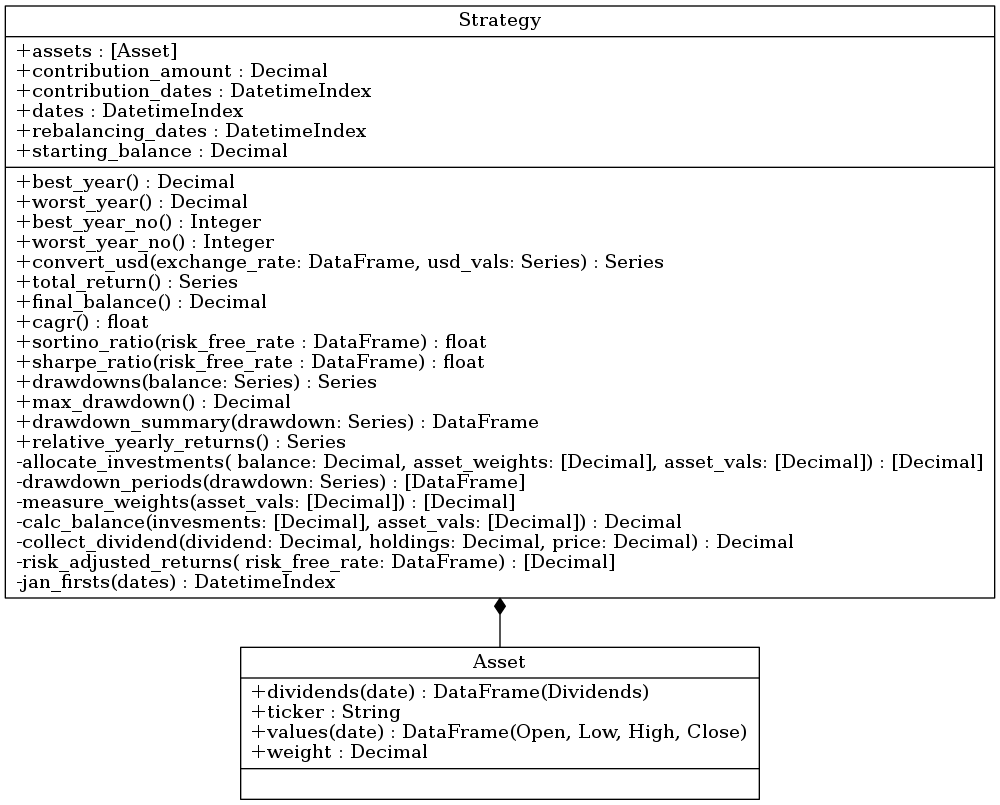
\includegraphics[width=\textwidth,keepaspectratio]{Report/08Appendices/084UML/084Pictures/classes_analyse_data.png}
   \caption{UML Diagrams - Anda}
\end{figure}

\subsection{Data Harvester}

\begin{figure}[H]
   \centering
   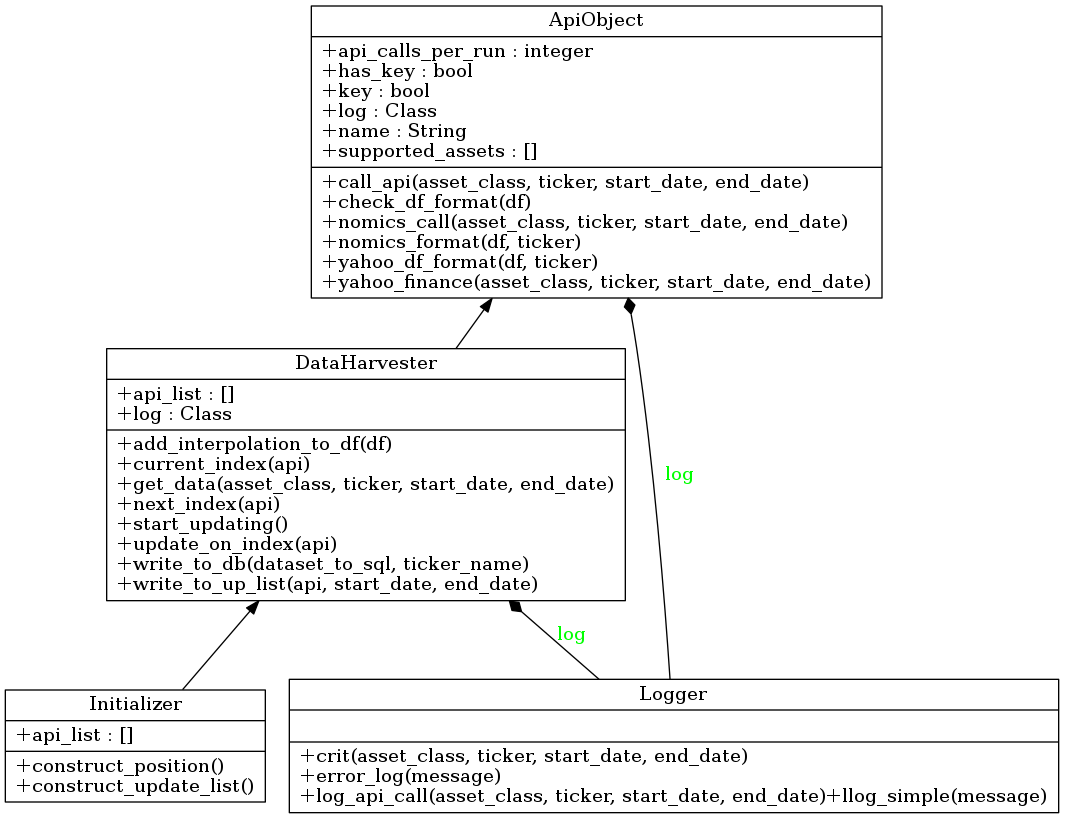
\includegraphics[width=\textwidth,keepaspectratio]{Report/08Appendices/084UML/084Pictures/classes_dhav_core_1.png}
   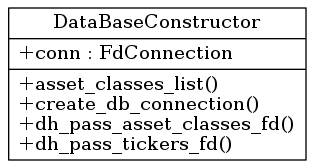
\includegraphics[scale=2.0,keepaspectratio]{Report/08Appendices/084UML/084Pictures/classes_dhav_core_2.png}
   \caption{UML Diagrams - Data Harvester}
\end{figure}

\subsection{Finda}

\begin{figure}[H]
   \centering
   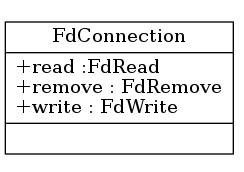
\includegraphics[scale=2.0,keepaspectratio]{Report/08Appendices/084UML/084Pictures/classes_Finda_1.png}
   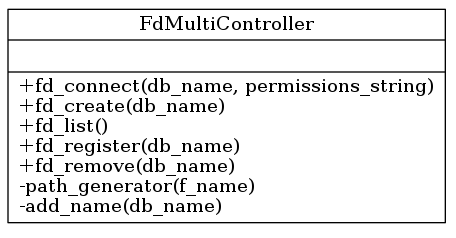
\includegraphics[scale=2.0,keepaspectratio]{Report/08Appendices/084UML/084Pictures/classes_Finda_2.png}
   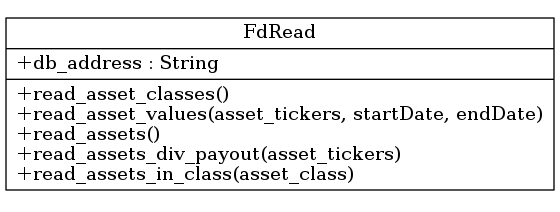
\includegraphics[scale=2.0,keepaspectratio]{Report/08Appendices/084UML/084Pictures/classes_Finda_3.png}
   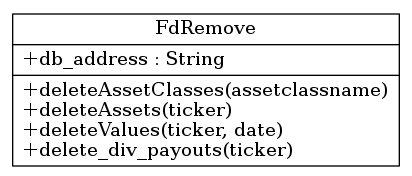
\includegraphics[scale=2.0,keepaspectratio]{Report/08Appendices/084UML/084Pictures/classes_Finda_4.png}
   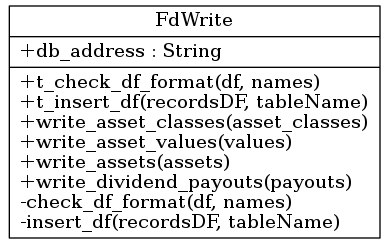
\includegraphics[scale=2.0,keepaspectratio]{Report/08Appendices/084UML/084Pictures/classes_Finda_5.png}
   \caption{UML Diagrams - Finda}
\end{figure}

\subsection{Thalia Web}

\begin{figure}[H]
   \centering
   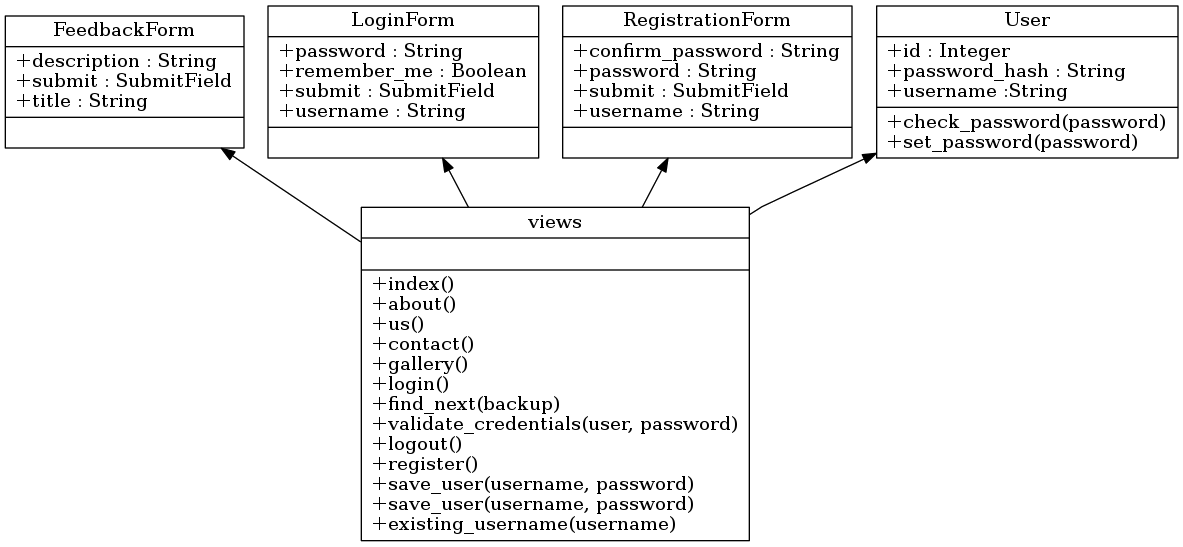
\includegraphics[width=\textwidth,keepaspectratio]{Report/08Appendices/084UML/084Pictures/classes_thalia_1.png}
   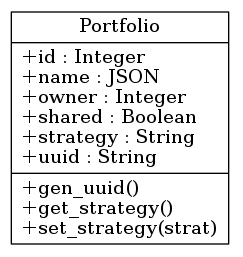
\includegraphics[scale=2.0,keepaspectratio]{Report/08Appendices/084UML/084Pictures/classes_thalia_2.png}
   \caption{UML Diagrams - Thalia Web}
\end{figure}

\end{document}
